% cone20-udf.tex

\section{Mach 1.5 flow over a 20-degree cone -- UDF boundaries}
\label{sec:cone20-udf}
%
This is a small (in both memory and run time) example 
that shows the implementation of user-defined boundary conditions.
It is otherwise equivalent to the case in Section\,\ref{cone20-simple-sec}.
Use the following commands:\\
%
\topbar\\
\texttt{\$ cd $\sim$/cfcfd3/examples/eilmer3/2D/cone20-udf}\\
\texttt{\$ ./cone20\_run.sh}\\
\bottombar\\
%
and, within a minute or so, you should end up with a number of files
with various solution data plotted.
The grid and initial solution are created and the time-evolution of the
flow field is computed for 5\,ms (with 1105 time steps being required).
The commands invoke the shell scripts displayed in 
subsection~\ref{cone20-udf-sh-files}.
%

\begin{figure}[htbp]
\begin{center}
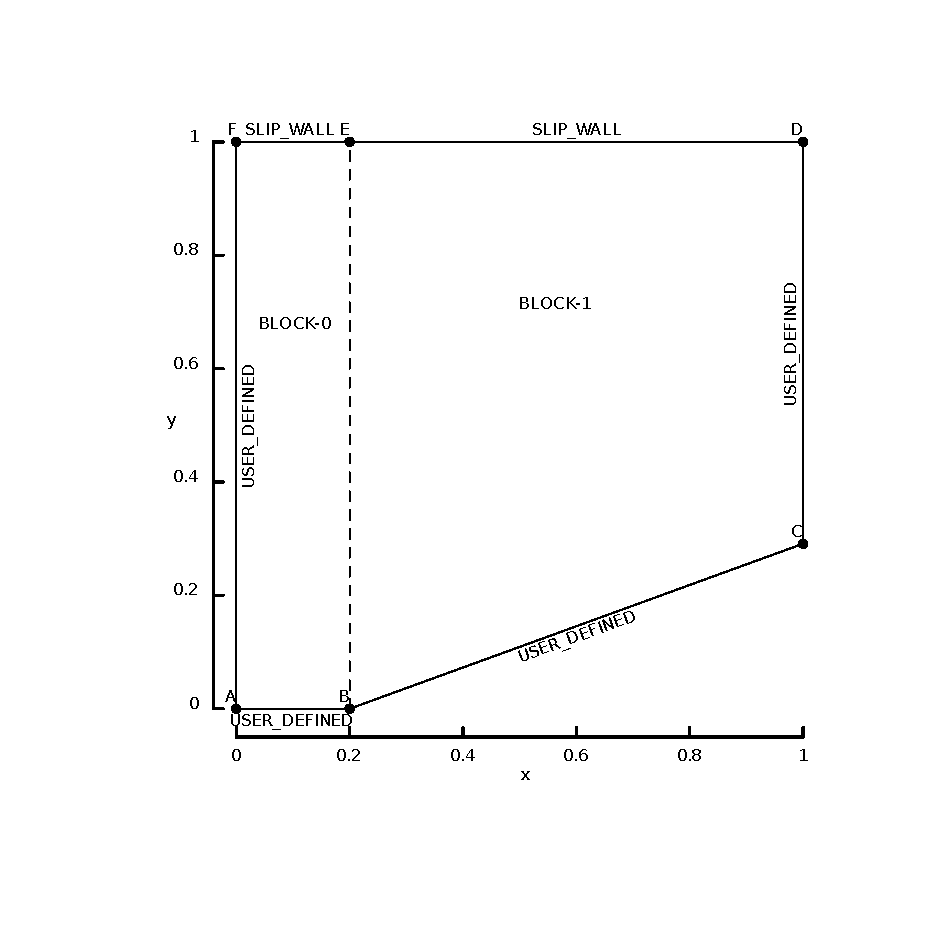
\includegraphics[width=10cm, viewport=76 78 389 398]{../2D/cone20-udf/cone20_svg.pdf}
\end{center}
\caption{Schematic diagram of the geometry for a cone 
         with 20 degree half-angle and user-defined boundaries.}
\label{cone20-udf-geometry-fig}
\end{figure}

\medskip
The free-stream conditions ($p_{\infty} = 95.84$\,kPa, $T_{\infty} = 1103$\,K
and $u_{\infty} = 1000$\,m/s) are related to the shock-over-ramp test problem
in the original ICASE Report\,\cite{jacobs_91d} and are set to give a 
Mach number of 1.5.
From Chart 5 in Ref.\,\cite{ames_53}, the expected steady-state shock wave
angle is 49$^o$ and, from Chart 6, the pressure coefficent is
$$
\frac{p_{cone-surface} - p_{\infty}}{q_{\infty}} \approx 0.387
$$
and the dynamic pressure for the specified free stream is
$q_{\infty} = \frac{1}{2} \rho_{\infty} u_{\infty}^2 \approx 151.38$\,kPa.
Figure~\ref{cone20-udf-axial-force-fig} shows the pressure coefficient 
estimated as
$$
C_p = \frac{f_x - p_{\infty} A}{q_{\infty} A}
$$
from the simulated axial force, $f_x$, written into the simulation log file
and frontal area of the cone, $A$.

\begin{figure}[htbp]
\begin{center}
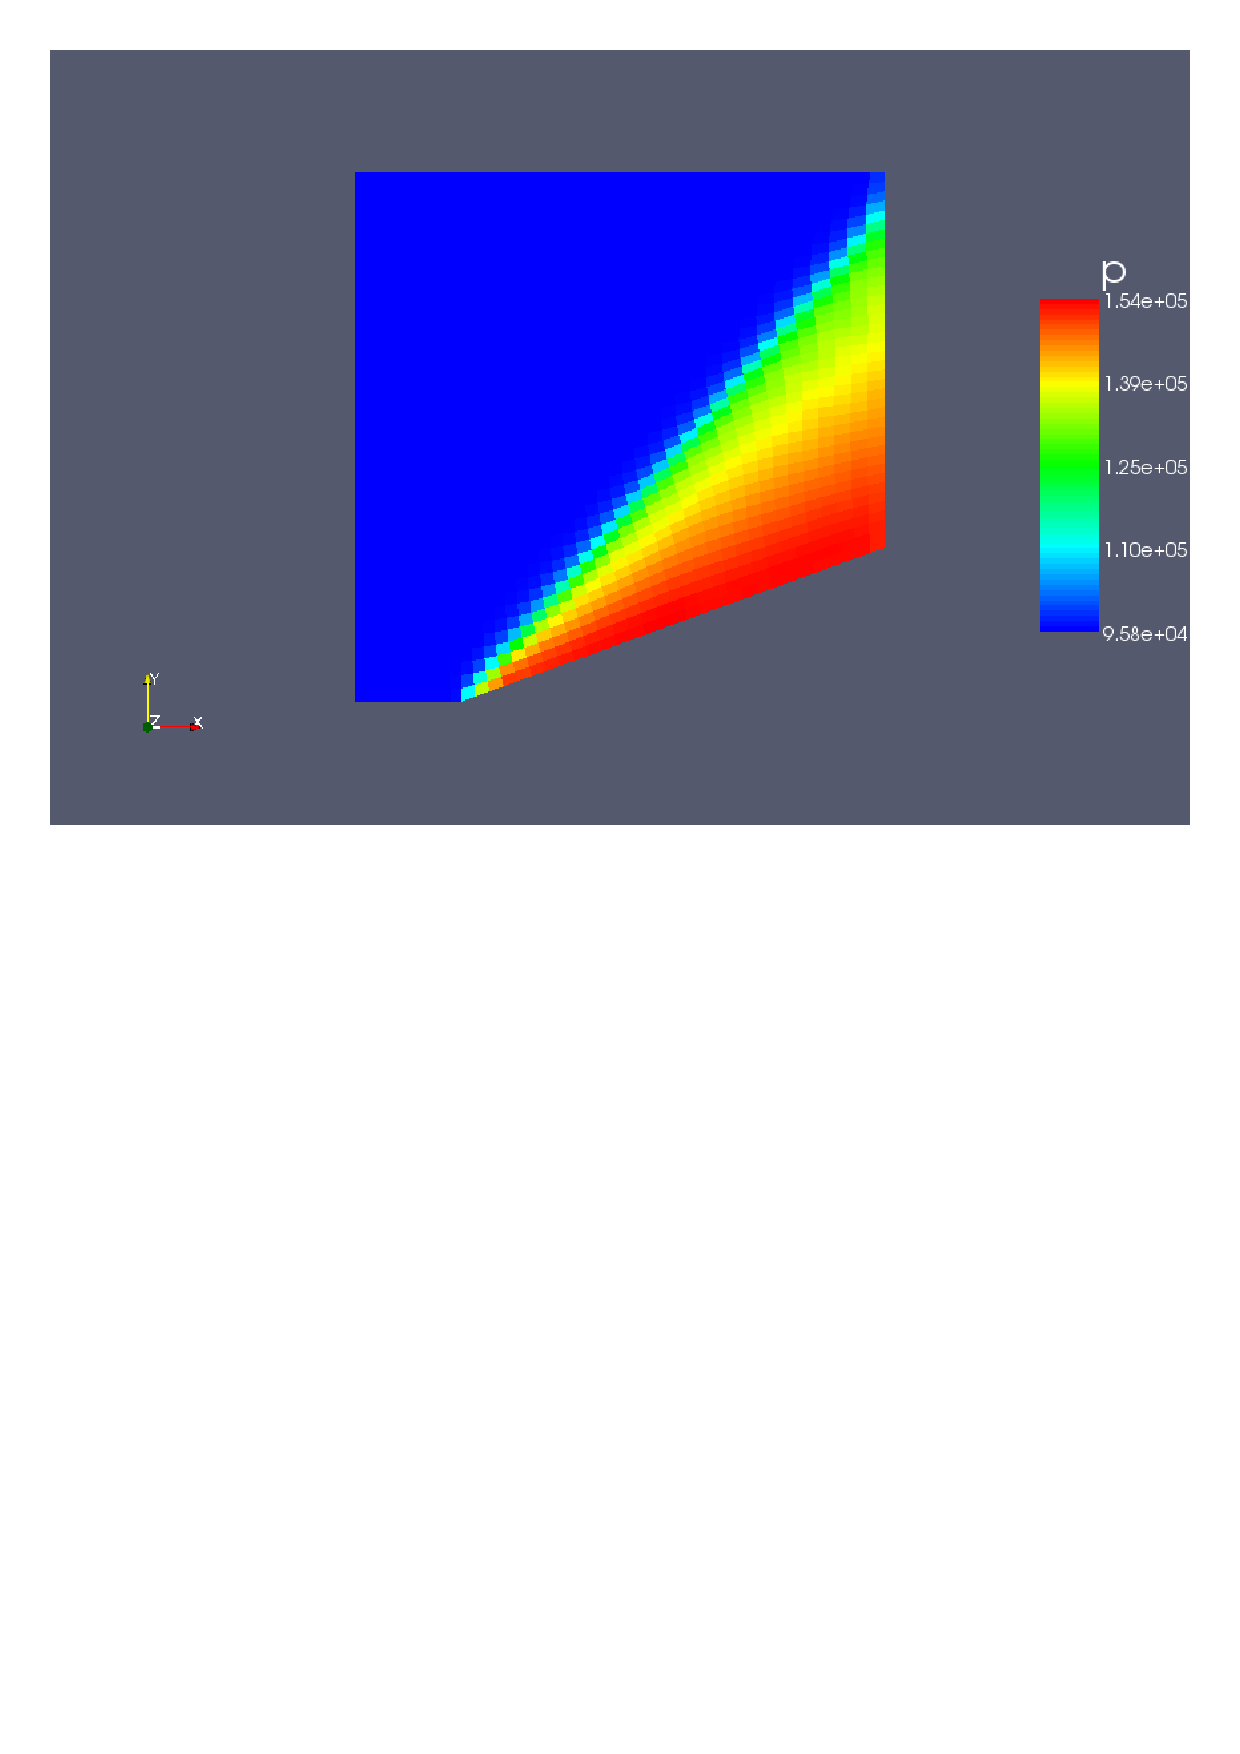
\includegraphics[width=0.8\textwidth, viewport=24 447 571 819]{../2D/cone20-udf/cone20_p.pdf}
\end{center}
\caption{Pressure data for flow over a cone with 20 degree half-angle.
         The shock profile is not yet straight and the pressure field
         near the cone surface is not conically symmetric, although it
	 would become more so if we continued the simulation.}
\label{cone20-udf-pressure-fig}
\end{figure}

\begin{figure}[htbp]
\begin{center}
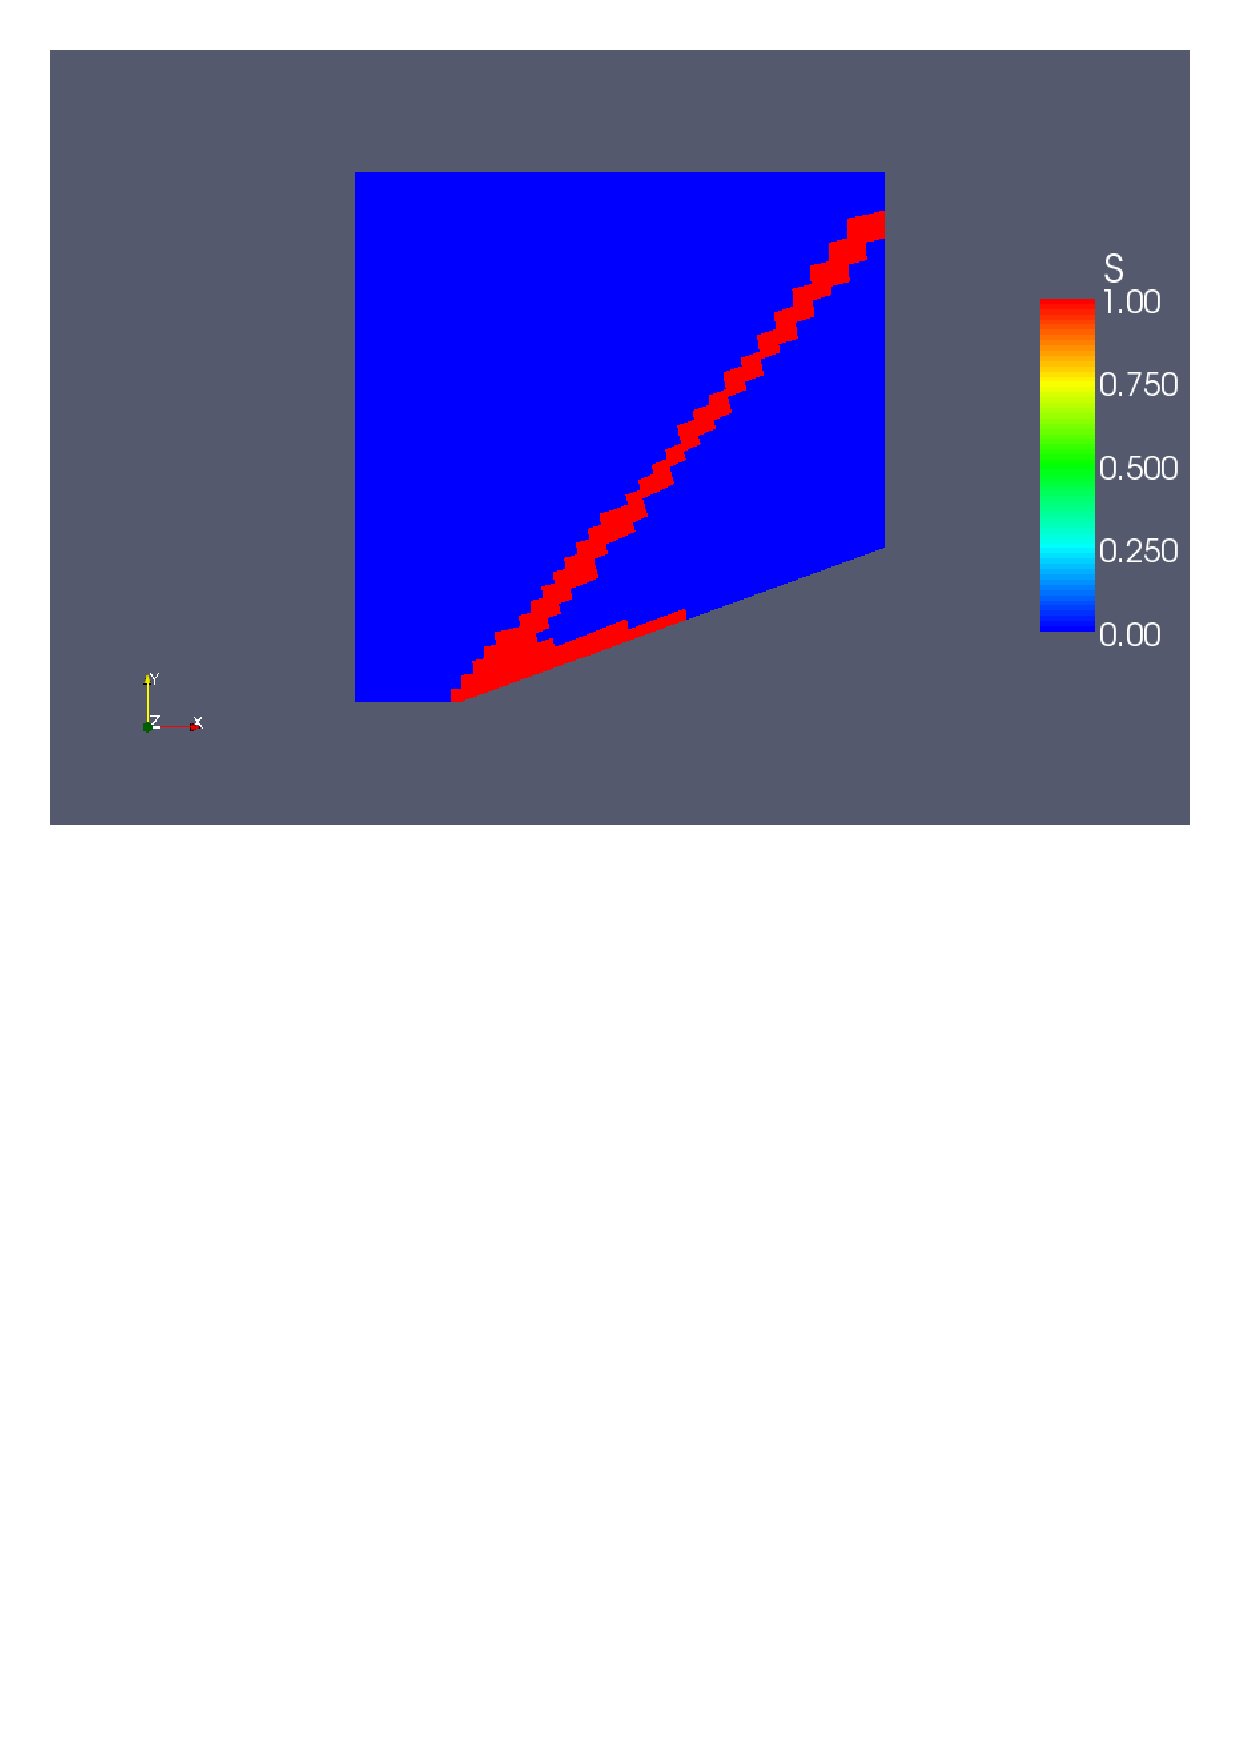
\includegraphics[width=0.8\textwidth, viewport=24 447 571 819]{../2D/cone20-udf/cone20_S.pdf}
\end{center}
\caption{Shock-sensor data for flow over a cone with 20 degree half-angle.
         For the \texttt{adaptive} flux calculator, 
	 this sensor indicates the regions
	 of the flow where the more dissipative scheme should be used.}
\label{cone20-udf-shock-sensor-fig}
\end{figure}

\begin{figure}[htbp]
\begin{center}
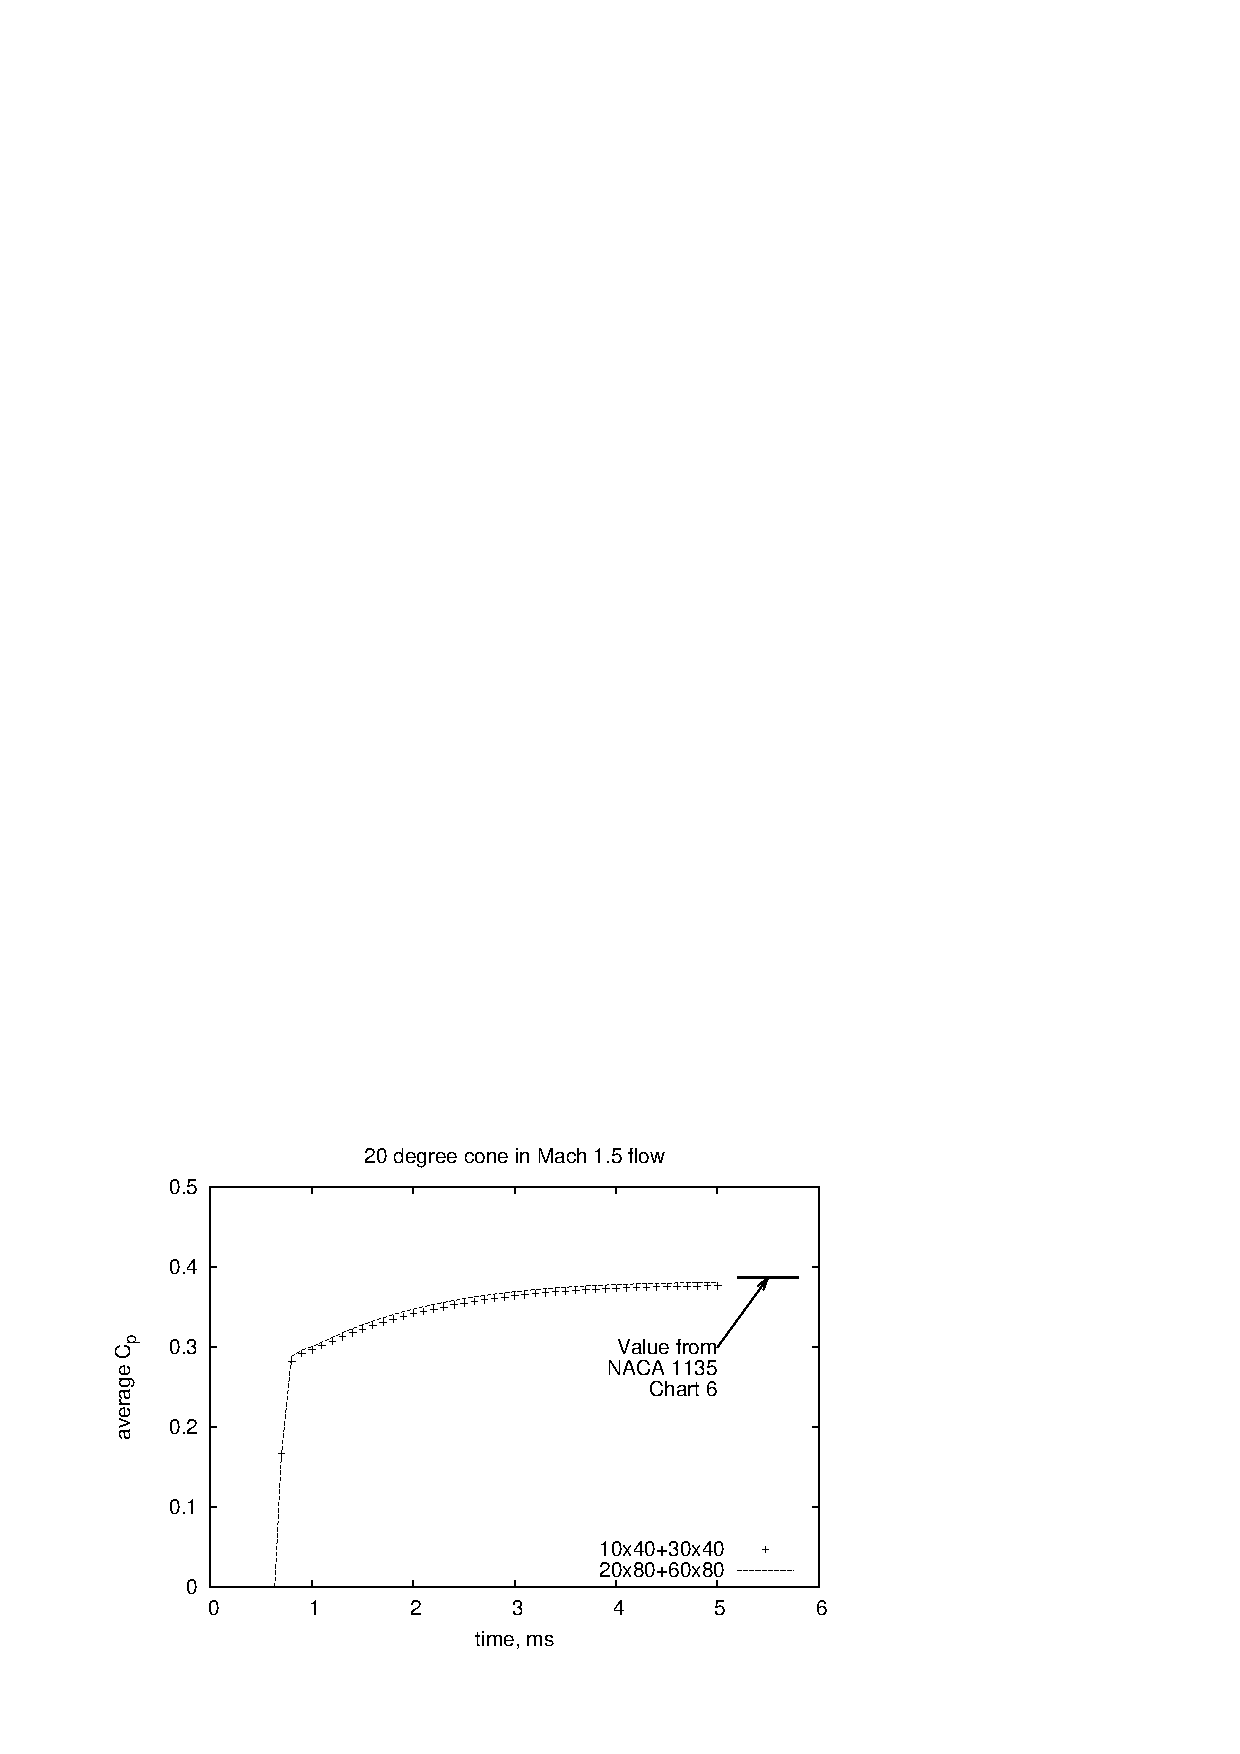
\includegraphics[width=10cm, viewport=52 49 401 294]{../2D/cone20-udf/cone20_cp.pdf}
\end{center}
\caption{Evolution of the axial (drag) force
         for flow over a cone with 20 degree half-angle
	 for two mesh resolutions.}
\label{cone20-udf-axial-force-fig}
\end{figure}

\newpage

\subsection{Input script (.py)}\index{boundary conditions!UserDefinedBC!example of use}
\topbar
\lstinputlisting[language={}]{../2D/cone20-udf/cone20.py}
\bottombar

\newpage
\subsection{Boundary-condition files (.lua)}
\topbar
\lstinputlisting[language={}]{../2D/cone20-udf/udf-supersonic-in.lua}
\bottombar \\
\topbar
\lstinputlisting[language={}]{../2D/cone20-udf/udf-extrapolate-out.lua}
\bottombar \\
\topbar
\lstinputlisting[language={}]{../2D/cone20-udf/udf-slip-wall.lua}
\bottombar \\
\topbar
\lstinputlisting[language={}]{../2D/cone20-udf/udf-process.lua}
\bottombar

\subsection{Shell scripts}
\label{cone20-udf-sh-files}
\topbar
\lstinputlisting[language={}]{../2D/cone20-udf/cone20_run.sh}
\bottombar

\subsection{Notes}
\begin{itemize}
\item Run time is approximately 94 seconds for 1126 steps on a computer with 
      an Intel Dual Pentium E2160, 1.6\,GHz processor.  
      As would be expected, the calling of the user-defined (Lua) functions
      carries some cost, but not much.
\end{itemize}
